\section{Interrupt}
\begin{frame}{Outline}
 \begin{description}
  \item[Callback] Hollywood Prizip: 
   \begin{quote}
    don't call us, we'll call you.
   \end{quote}
   \vspace{-7mm}
   \begin{itemize}
    \item die Hardware ruft zur�ck
   \end{itemize}
  \item[Interrupts] Der Schritt zur Echtzeit
  \begin{itemize}
   \item Die Hardware ruft Software auf
   \item Elementare Anwendung vom {\em callback}
   \item Ereignisgesteuert: {\em event driven}
  \end{itemize}
 \end{description}
\end{frame}

\begin{frame}{SW braucht HW}{und umgekehrt}
\begin{center}
 
\includegraphics[width=0.75\textwidth]{hw-sw-calls.pdf}
\end{center}
 \begin{block}{Beispiel}
  \begin{description}
   \item[SW$\to$HW]
    \begin{itemize}
     \item Setze LED
     \item Schreibe Buchstabe 
    \end{itemize}
    \item[HW$\to$SW]
     \begin{itemize}
      \item Ein {\em timer} tick
      \item Tastatur Taste gedr�ckt
     \end{itemize}
  \end{description}
 \end{block}
 \vspace{-5mm}
 \remark{Beide Richtungen {\em SW$\to$HW} und {\em HW$\to$SW} sind wichtig}
\end{frame}

\begin{frame}{Asynchron}{jederzeit}
\begin{block}{Normale Programmausf�hrung: Thread}
\begin{center}
 
\includegraphics[width=0.5\textwidth]{thread.pdf}
\end{center}
\end{block}
\vspace{-5mm}
\begin{block}{Interrupt}
 \vspace{-5mm}
  \begin{center}
 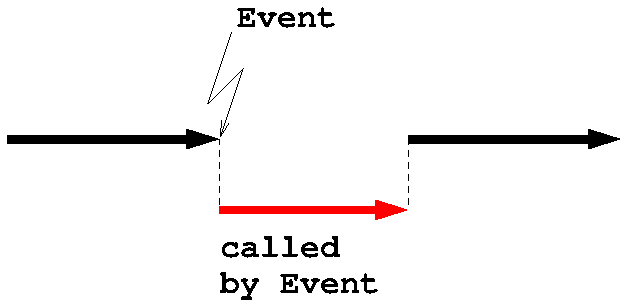
\includegraphics[width=0.5\textwidth]{interrupted-thread.pdf}
 \end{center}
\end{block} 
\vspace{-5mm}
\begin{description}[unsichtbar]
 \item[jederzeit] Zwischen zwei Instruktionen
 \item[unsichtbar] vom Thread aus gesehen
\end{description}
\end{frame}

\begin{frame}{Informationen}
 \begin{itemize}
  \item \cod{cat /proc/interrupts}
 \end{itemize}
\end{frame}

\subsection{gpio-2.c}
\begin{frame}{Ziel}
 \begin{itemize}
  \item Interrupt erkennen
  \item Switch
  \begin{itemize}
   \item dr�cken: erzeugt interrupt: \cod{IRQF\_TRIGGER\_RISING}
   \item loslassen: erzeugt interrupt:\cod{IRQF\_TRIGGER\_FALLING}
  \end{itemize}
 \end{itemize}
\end{frame}

\begin{frame}[fragile]{gpio-2.c}{schrittweise}
 \begin{itemize}
  \item \href{https://elixir.bootlin.com/linux/latest/source/include/linux/gpio.h\#L147}
             {\cod{gpio\_direction\_input}}
  \item \href{https://elixir.bootlin.com/linux/latest/source/include/linux/gpio.h\#L216}
             {\cod{gpio\_to\_irq}}
  \item \href{https://elixir.bootlin.com/linux/latest/source/include/linux/interrupt.h\#L146}
             {\cod{request\_irq}}    
 \end{itemize}
 \begin{block}{Der Handler}
\begin{lstlisting}
static  irqreturn_t onSWI(int id,void* d)
{
 printk("onSWI\n"); /* debug */
 /* do something */
 return IRQ_HANDLED;
}
\end{lstlisting}
 \end{block}
\end{frame}

